%%%%%%%%%%%%%%%%%%%%%%%%%%%%%%%%%%%%%%%%%%%%%%%%%%%%%%%%%%%%%%%%%%%%%%%%%%%%%%%%
%Tutorial slides on Python.
%
% Author: FOSSEE
% Copyright (c) 2009, FOSSEE, IIT Bombay
%%%%%%%%%%%%%%%%%%%%%%%%%%%%%%%%%%%%%%%%%%%%%%%%%%%%%%%%%%%%%%%%%%%%%%%%%%%%%%%%

\documentclass[14pt,compress]{beamer}
%\documentclass[draft]{beamer}
%\documentclass[compress,handout]{beamer}
%\usepackage{pgfpages} 
%\pgfpagesuselayout{2 on 1}[a4paper,border shrink=5mm]

% Modified from: generic-ornate-15min-45min.de.tex
\mode<presentation>
{
  \usetheme{Warsaw}
  \useoutertheme{split}
  \setbeamercovered{transparent}
}

\usepackage[english]{babel}
\usepackage[latin1]{inputenc}
%\usepackage{times}
\usepackage[T1]{fontenc}

% Taken from Fernando's slides.
\usepackage{ae,aecompl}
\usepackage{mathpazo,courier,euler}
\usepackage[scaled=.95]{helvet}
\usepackage{amsmath}

\definecolor{darkgreen}{rgb}{0,0.5,0}

\usepackage{listings}
\lstset{language=Python,
    basicstyle=\ttfamily\bfseries,
    commentstyle=\color{red}\itshape,
  stringstyle=\color{darkgreen},
  showstringspaces=false,
  keywordstyle=\color{blue}\bfseries}

%%%%%%%%%%%%%%%%%%%%%%%%%%%%%%%%%%%%%%%%%%%%%%%%%%%%%%%%%%%%%%%%%%%%%%
% Macros
\setbeamercolor{emphbar}{bg=blue!20, fg=black}
\newcommand{\emphbar}[1]
{\begin{beamercolorbox}[rounded=true]{emphbar} 
      {#1}
 \end{beamercolorbox}
}
\newcounter{time}
\setcounter{time}{0}
\newcommand{\inctime}[1]{\addtocounter{time}{#1}{\tiny \thetime\ m}}

\newcommand{\typ}[1]{\lstinline{#1}}

\newcommand{\kwrd}[1]{ \texttt{\textbf{\color{blue}{#1}}}  }

%%% This is from Fernando's setup.
% \usepackage{color}
% \definecolor{orange}{cmyk}{0,0.4,0.8,0.2}
% % Use and configure listings package for nicely formatted code
% \usepackage{listings}
% \lstset{
%    language=Python,
%    basicstyle=\small\ttfamily,
%    commentstyle=\ttfamily\color{blue},
%    stringstyle=\ttfamily\color{orange},
%    showstringspaces=false,
%    breaklines=true,
%    postbreak = \space\dots
% }

%%%%%%%%%%%%%%%%%%%%%%%%%%%%%%%%%%%%%%%%%%%%%%%%%%%%%%%%%%%%%%%%%%%%%%
% Title page
\title[]{Least Squares Fit\\Statistical Plotting}

\author[FOSSEE] {FOSSEE}

\institute[IIT Bombay] {Department of Aerospace Engineering\\IIT Bombay}
\date[] {31, October 2009\\Day 1, Session 3}
%%%%%%%%%%%%%%%%%%%%%%%%%%%%%%%%%%%%%%%%%%%%%%%%%%%%%%%%%%%%%%%%%%%%%%

%\pgfdeclareimage[height=0.75cm]{iitmlogo}{iitmlogo}
%\logo{\pgfuseimage{iitmlogo}}


%% Delete this, if you do not want the table of contents to pop up at
%% the beginning of each subsection:
\AtBeginSubsection[]
{
  \begin{frame}<beamer>
    \frametitle{Outline}
    \tableofcontents[currentsection,currentsubsection]
  \end{frame}
}

\AtBeginSection[]
{
  \begin{frame}<beamer>
    \frametitle{Outline}
    \tableofcontents[currentsection,currentsubsection]
  \end{frame}
}

\newcommand{\num}{\texttt{numpy}}


% If you wish to uncover everything in a step-wise fashion, uncomment
% the following command: 
%\beamerdefaultoverlayspecification{<+->}

%\includeonlyframes{current,current1,current2,current3,current4,current5,current6}

%%%%%%%%%%%%%%%%%%%%%%%%%%%%%%%%%%%%%%%%%%%%%%%%%%%%%%%%%%%%%%%%%%%%%%
% DOCUMENT STARTS
\begin{document}

\begin{frame}
  \maketitle
\end{frame}

%% \begin{frame}
%%   \frametitle{Outline}
%%   \tableofcontents
%%   % You might wish to add the option [pausesections]
%% \end{frame}

\begin{frame}
  \frametitle{More on data processing}
  \begin{block}{}
    What do we do if we want to draw Pie charts for the data in a huge data file?
  \end{block}
\end{frame}


\begin{frame}
  \frametitle{Statistical Analysis and Parsing}
  Read the data supplied in \emph{sslc1.txt} and obtain the following statistics:
  \begin{itemize}
    \item Draw a pie chart representing the number of students who scored more than 90\% in Science per region.
    \item Draw a pie chart representing the number of students who scored more than 90\% per subject(All regions combined).
  \end{itemize}
\end{frame}

\begin{frame}
  \frametitle{Statistical Analysis and Parsing \ldots}
  Machinery Required -
  \begin{itemize}
    \item File reading and parsing
    \item Dictionaries
  \end{itemize}
\end{frame}

\begin{frame}
  \frametitle{File reading and parsing}
  Understanding the structure of sslc1.txt
  \begin{itemize}
    \item Each line in the file, i.e each row of a file is a single record.
    \item Each record corresponds to a record of a single student
    \item Each record consists of several fields separated by a ';'
  \end{itemize}
\end{frame}

\begin{frame}
  \frametitle{File reading and parsing \ldots}
  Each record consists of:
  \begin{itemize}
    \item Region Code
    \item Roll Number
    \item Name
    \item Marks of 5 subjects
    \item Total marks
    \item Pass (P)
    \item Withdrawn (W)
    \item Fail (F)
  \end{itemize}
\end{frame}

\begin{frame}[fragile]
  \frametitle{File reading and parsing \ldots}
  \begin{lstlisting}
for record in open('sslc1.txt'):
    fields = record.split(';')
  \end{lstlisting}
\end{frame}

\begin{frame}[fragile]
  \frametitle{Dictionary - Building parsed data}
  \begin{itemize}
    \item Let the parsed data be stored in list of dictionaries.
    \item d = \{\} is an empty dictionary
  \end{itemize}
\end{frame}

\begin{frame}[fragile]
  \frametitle{Dictionary - Building parsed data}
\begin{lstlisting}
ninety_percents = [{}, {}, {}, {}, {}]
\end{lstlisting}
\end{frame}

\begin{frame}[fragile]
  \frametitle{Dictionary - Building parsed data}
  \begin{itemize}
    \item Index of a dictionary is called a \emph{key}
    \item \emph{Keys} of these dictionaries are strings - region codes
  \end{itemize}
\end{frame}

\begin{frame}[fragile]
  \frametitle{Dictionary - Building parsed data \ldots}
  \begin{itemize}
    \item Value of a \emph{key} can be any legal Python value
    \item In this problem let the value of a \emph{key} be another an integer
    \item This dictionary contains:
  \end{itemize}
'region code': Number of students who scored more than 90\% in this region for this subject
\end{frame}

\begin{frame}[fragile]
  \frametitle{Building parsed data \ldots}
  \begin{lstlisting}
from pylab import *

ninety_percents = [{}, {}, {}, {}, {}]

for record in open('sslc1.txt'):
    record = record.strip()
    fields = record.split(';')

    region_code = fields[0].strip()
  \end{lstlisting}
\end{frame}

\begin{frame}[fragile]
  \frametitle{Building parsed data \ldots}
  \small
  \begin{lstlisting}
for i, field in enumerate(fields[3:8]):

    if region_code not in ninety_percents[i]:
        ninety_percents[i][region_code] = 0

    score_str = field.strip()

    score = 0 if score_str == 'AA' else 
                         int(score_str)
    if score > 90:
        ninety_percents[i][region_code] += 1
  \end{lstlisting}
\end{frame}

\begin{frame}[fragile]
  \frametitle{Consolidating data}
  \begin{lstlisting}
subj_total = []
for subject in ninety_percents:
    subj_total.append(sum(
         subject.values()))
  \end{lstlisting}
\end{frame}

\begin{frame}[fragile]
  \frametitle{Pie charts}
  \small
  \begin{lstlisting}
figure(1)
pie(ninety_percents[4].values(), 
    labels=ninety_percents[1].keys())
title('Students scoring 90% and above 
      in science by region')
savefig('/tmp/science.png')
  \end{lstlisting}
\begin{columns}
    \column{5.25\textwidth}
    \hspace*{1.1in}
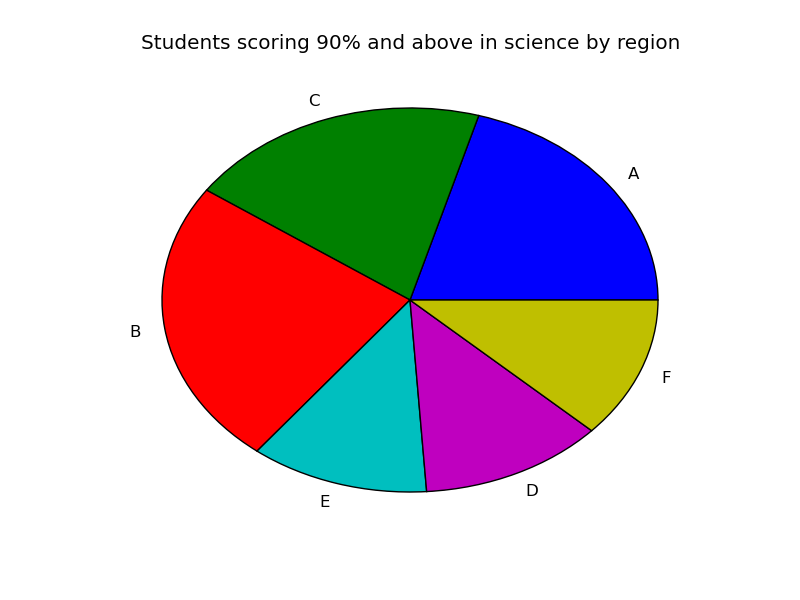
\includegraphics[height=2in, interpolate=true]{data/science}
    \column{0.8\textwidth}
\end{columns}
\end{frame}

\begin{frame}[fragile]
  \frametitle{Pie charts}
  \begin{lstlisting}
figure(2)
pie(subj_total, labels=['English',
    'Hindi', 'Maths', 'Science',
    'Social'])
title('Students scoring more than
      90% by subject(All regions
      combined).')
savefig('/tmp/all_regions.png')
  \end{lstlisting}
\end{frame}

\begin{frame}[fragile]
  \frametitle{Pie charts}
  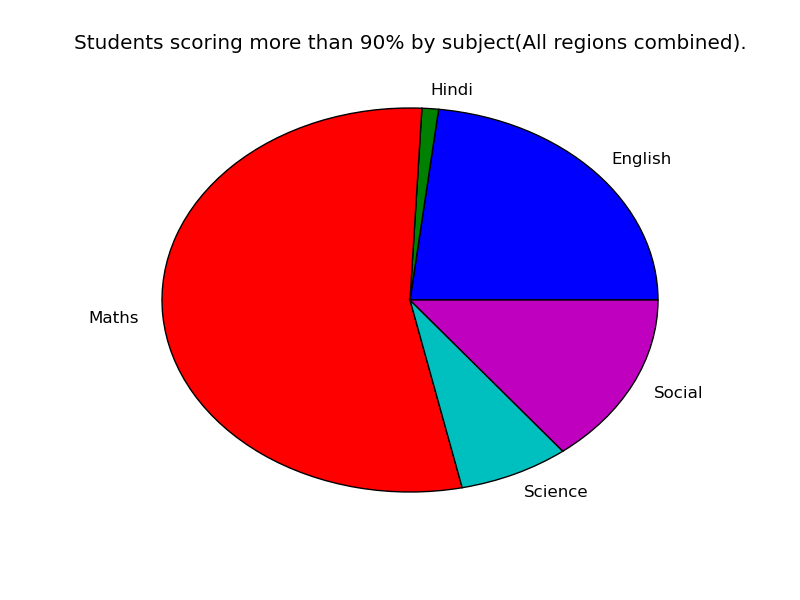
\includegraphics[height=3in, interpolate=true]{data/all_regions}
\end{frame}

\begin{frame}[fragile]
\frametitle{Dealing with data whole-sale}
\begin{lstlisting}
In []: for t in T:
 ....:     Tsq.append(t*t)
\end{lstlisting}
\begin{itemize}
\item This is not very efficient
\item We are squaring element after element
\item We use arrays to make this efficient
\end{itemize}
\begin{lstlisting}
In []: L = array(L)
In []: T = array(T)
In []: Tsq = T*T
\end{lstlisting}
\end{frame}

\begin{frame}[fragile]
\frametitle{Arrays}
\begin{itemize}
\item \typ{T} and \typ{L} are now arrays
\item arrays are very efficient and powerful 
\item Very easy to perform element-wise operations
\item \typ{+, -, *, /, \%}
\item More about arrays later
\end{itemize}
\end{frame}

\begin{frame}[fragile]
\frametitle{Least Squares Fit}
\vspace{-0.15in}
\begin{figure}
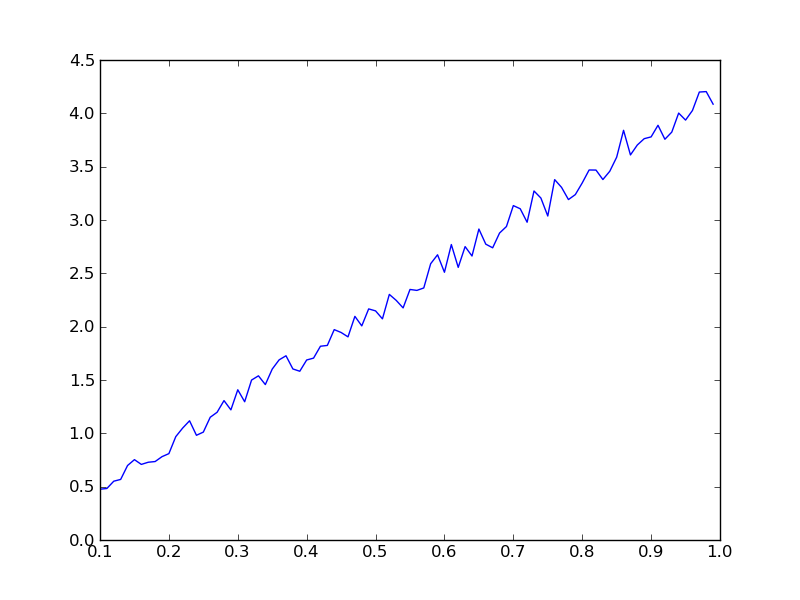
\includegraphics[width=4in]{data/L-Tsq-Line.png}
\end{figure}
\end{frame}

\begin{frame}[fragile]
\frametitle{Least Squares Fit}
\vspace{-0.15in}
\begin{figure}
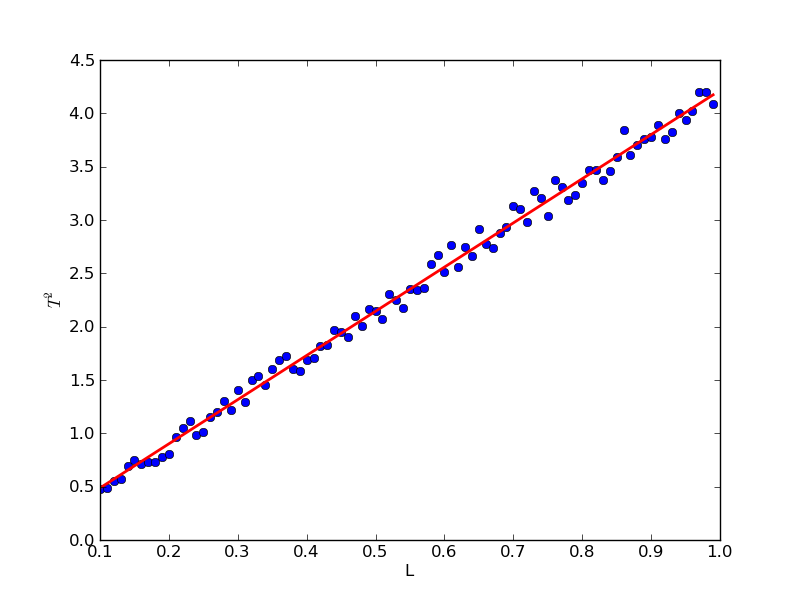
\includegraphics[width=4in]{data/least-sq-fit.png}
\end{figure}
\end{frame}

\begin{frame}
\frametitle{Least Square Fit Curve}
\begin{itemize}
\item $T^2$ and $L$ have a linear relationship
\item Hence, Least Square Fit Curve is a line
\item we shall use the \typ{lstsq} function
\end{itemize}
\end{frame}

\begin{frame}[fragile]
\frametitle{\typ{lstsq}}
\begin{itemize}
\item We need to fit a line through points for the equation $T^2 = m \cdot L+c$
\item The equation can be re-written as $T^2 = A \cdot p$
\item where A is   
  $\begin{bmatrix}
  L_1 & 1 \\
  L_2 & 1 \\
  \vdots & \vdots\\
  L_N & 1 \\
  \end{bmatrix}$
  and p is 
  $\begin{bmatrix}
  m\\
  c\\
  \end{bmatrix}$
\item We need to find $p$ to plot the line
\end{itemize}
\end{frame}

\begin{frame}[fragile]
\frametitle{Van der Monde Matrix}
\begin{itemize}
\item A is also called a Van der Monde matrix
\item It can be generated using \typ{vander}
\end{itemize}
Van der Monde matrix of order M
\begin{equation*}
  \begin{bmatrix}
  l_1^{M-1} & \ldots & l_1 & 1 \\
  l_2^{M-1} & \ldots &l_2 & 1 \\
  \vdots & \ldots & \vdots & \vdots\\
  l_N^{M-1} & \ldots & l_N & 1 \\
  \end{bmatrix}
\end{equation*}
\begin{lstlisting}
In []: A = vander(L,2)
\end{lstlisting}
\end{frame}

\begin{frame}[fragile]
\frametitle{\typ{lstsq} \ldots}
\begin{itemize}
\item Now use the \typ{lstsq} function
\item Along with a lot of things, it returns the least squares solution
\end{itemize}
\begin{lstlisting}
In []: coef, res, r, s = lstsq(A,Tsq)
\end{lstlisting}
\end{frame}

\begin{frame}[fragile]
\frametitle{Least Square Fit Line \ldots}
We get the points of the line from \typ{coef}
\begin{lstlisting}
In []: Tline = coef[0]*L + coef[1]
\end{lstlisting}
\begin{itemize}
\item Now plot Tline vs. L, to get the Least squares fit line. 
\end{itemize}
\begin{lstlisting}
In []: plot(L, Tline)
\end{lstlisting}
\end{frame}

\begin{frame}[fragile]
  \frametitle{What did we learn?}
  \begin{itemize}
   \item Dictionaries
   \item Drawing pie charts
  \end{itemize}
\end{frame}
\end{document}
